\documentclass[10pt,showpacs,preprintnumbers,amsmath,amssymb,nofootinbib,aps,prl,twocolumn,groupedaddress,superscriptaddress,showkeys]{revtex4-1}
\usepackage{graphicx}
\usepackage{dcolumn}
\usepackage{bm}
\usepackage[colorlinks=true,urlcolor=blue,citecolor=blue]{hyperref}
\usepackage{color}
\usepackage{listings}
\usepackage{subfig}
\usepackage{float}
\usepackage{tikz} % Send help 
  \usetikzlibrary{automata, positioning}
\usepackage{physics}

\lstset{ %
  basicstyle=\footnotesize,        % the size of the fonts that are used for the code
  breakatwhitespace=false,         % sets if automatic breaks should only happen at whitespace
  breaklines=true,                 % sets automatic line breaking
  captionpos=t,                    % sets the caption-position to bottom
  deletekeywords={...},            % if you want to delete keywords from the given language
  escapeinside={\%*}{*)},          % if you want to add LaTeX within your code
  extendedchars=true,              % lets you use non-ASCII characters; for 8-bits encodings only, does not work with UTF-8
  frame=single,                    % adds a frame around the code
  keepspaces=true,                 % keeps spaces in text, useful for keeping indentation of code (possibly needs columns=flexible)
 % language=Python,                 % the language of the code
  morekeywords={*,...},           % if you want to add more keywords to the set
  numbers=left,                    % where to put the line-numbers; possible values are (none, left, right)
  numbersep=5pt,                   % how far the line-numbers are from the code
  showspaces=false,                % show spaces everywhere adding particular underscores; it overrides 'showstringspaces'
  showstringspaces=false,          % underline spaces within strings only
  showtabs=false,                  % show tabs within strings adding particular underscores
  stepnumber=1,                    % the step between two line-numbers. If it's 1, each line will be numbered
  tabsize=2,                       % sets default tabsize to 2 spaces
}

\captionsetup[subfigure]{labelformat=brace}

\begin{document}
\title{Disease Modeling - FYS3150 Computational Physics}
\author{Nicholas Karlsen}


\begin{abstract}
\end{abstract}

\maketitle


\section{Introduction}

\section{Theory, Algorithms and Methods}  
  \subsection{Runge-Kutta methods}
    

  \subsection{\label{sec:Markov Chains}Markov Chains}
    A Markov Chain aims to model the behavior of stochastic processes, that is models which time-evolution of each parameter $x_i$ is governed by a set of transition probabilities $P(x_i \rightarrow x_j)$.

    The k-th state of the system is given by the state vector $\vb x_k$, a column vector with entries $x_i$ for each parameter of the system.
      \begin{equation}
        \vb x_k = \mqty(x_1 \\ \vdots \\ x_i \\ \vdots \\ x_n)
      \end{equation}
    The transition probabilities $P(x_i\rightarrow x_j)$ are contained within a Stochastic matrix, $M$, an $n\times n$ matrix which columns are probability vectors that sum to unity. $M$ is such that multiplying it by a state $\vb x_k$ determines the next state, $\vb x_{k+1}$
      \begin{equation}
        M \vb x_k = \vb x_{k+1}
      \end{equation}


    From Theorem 18 in \textcite[p.~277]{linalg_lays}, if $M$ is a regular stochastic matrix there exists a unique steady state vector $\vb q$ which the system will converge towards as $k\rightarrow \infty$ characterized by
    \begin{equation}
      \vb x_k = \vb x_{k+1} 
    \end{equation}
    Regardless of the initial state, $\vb x_0$.

  \subsection{SIRS Model}

    The SIRS model is a type of mathematical model describing how infectious disease evolves within a population, and is a part of a family of similar models in epidemiology with various different features. In the SIRS model, the total population (N) is divided into three groups

    \begin{itemize}
      \item Susceptible (S) : People who do not have the disease, and are not immune to it.
      \item Infected (I) : People who are infected with the disease.
      \item Recovered (R) : People who has recovered from the infection, and have developed immunity.
    \end{itemize}

    Where the permitted traversal from one group to another follows a cyclical pattern $S \rightarrow I \rightarrow R \rightarrow S$.

    The rate of traversal is governed by a set of coupled differential equations,

    \begin{align}
      \begin{split}
        S' &= cR - \frac{aSI}{N} \\
        I' &= \frac{aSI}{N} - bI \\
        R' &= bI - cR 
        \label{eqn:transition rates}
      \end{split}
    \end{align}
    Where the constants $a,b,c$ are governing the

    \begin{itemize}
      \item rate of transmission
      \item rate of recovery
      \item rate of immunity loss
    \end{itemize}

    respectively, with dimension inverse time. For the purposes of this report, we will not consider a specific unit of time, but rather the dynamics of the system, as the timescales at which different diseases operate on vary. However, based on data (INSERT CITATIONS) a lot of common diseases are observed to operate on a scale of days, whilst some operate on a scale of years. 

    This system can also be modelled as a Stochastic system described as a Markov Chain, shown as a Markov diagram in Fig.~\ref{fig:SIRS diagram}. If we consider a small, finite timeinterval $\Delta t$, we can approximate the transition probabilities $P(x_i \rightarrow x_j)$ from Eqn.~\ref{eqn:transition rates}

    \begin{align}
      \begin{split}
        P(S\rightarrow I) &= \frac{aSI}{N}\Delta t
          \\
        P(I\rightarrow R) &= bI\Delta t
          \\
        P(R\rightarrow S) &= cR\Delta t
      \end{split}
    \end{align}
    It follows then, that the system will reach a steady state after a finite number of transitions for any set of initial conditions as discussed in Section~\ref{sec:Markov Chains}

    \subsubsection{Units}
     Units of time, and the rates $a,b,c, \dots$ isn't something i will pay much attention to in this report, as it is an entirely separate topic on it's own. And ultimately, would be decided on a per-disease basis. But for the sake of discussion, and exploration of the model, i will consider the time-scale of order $\approx$ years.

    \begin{figure}[h!tb]
      \centering 
      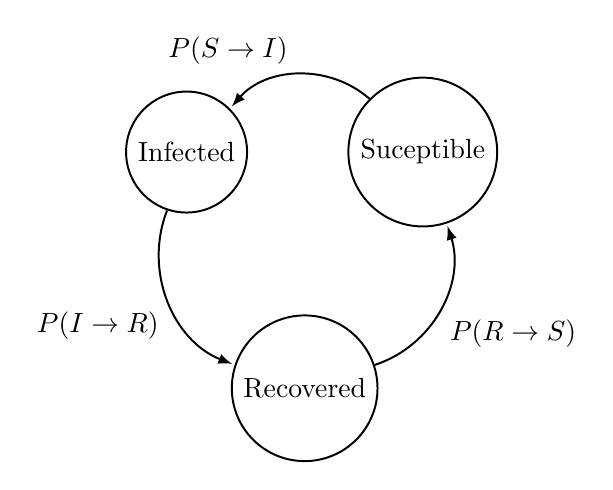
\begin{tikzpicture}
 
        % Setup the style for the states
        \tikzset{node style/.style={state, 
                                    minimum width=1.5cm,
                                    line width=.25mm
                                    }}
 
        % Draw the states
        \node[node style] at (3, 0)     (Suceptible)     {Suceptible};
        \node[node style] at (0, 0)     (Infected)     {Infected};
        \node[node style] at (1.5, -3) (Recovered) {Recovered};
 
        % Connect the states with arrows
        \draw[every loop,
              auto=right,
              line width=.25mm,
              >=latex]
            (Suceptible)    edge[bend right=45]  node {$P(S\rightarrow I)$} (Infected)
            (Infected)      edge[bend right=45]  node {$P(I\rightarrow R)$} (Recovered)
            (Recovered)     edge[bend right=45]  node {$P(R\rightarrow S)$} (Suceptible);
      \end{tikzpicture}
       \caption{The SIRS Model\label{fig:SIRS diagram}}
    \end{figure}

  \subsection{Monte-Carlo Algorithm}

  The Monte-Carlo way of simulating the various SIRS-Models are outlined in the following
  for the simplest case
\begin{lstlisting}[mathescape=true, language=python, title=SIRS Monte-Carlo]
for each $\textbf{MC-Cycle}$:
  for each $t_i$:
    Compute $P(S\rightarrow I)$
    Compute $P(I\rightarrow R)$
    Compute $P(R\rightarrow S)$

    if $P(S\rightarrow I)> r$ and $S_i > 0$:
      $S_{i+1}$ -= 1
      $I_{i+1}$ += 1

    if $P(I\rightarrow R)> r$ and $I_i > 0$:
      $I_{i+1}$ -= 1
      $R_{i+1}$ += 1

    if $P(R\rightarrow S)> r$ and $R_i > 0$:
      $R_{i+1}$ -= 1
      $S_{i+1}$ += 1
\end{lstlisting}
  
  We note here, a problem in the algorithm. That is; in what order do we evaluate the probabilities?
  Whether to consider $P(S\rightarrow I)$ or P$(R\rightarrow S)$ first is completely arbitrary, but may lead to a certain bias in smaller populations or when a group is nearing the lower limit of 0.

  Another important issue, that is dealt with in the IF statements is the potential of negative population groups. Whilst the overall net population is easily conserved\footnote{Mathematically, anyway.}, we have to ensure that no groups goes below 0. This can be done in one of two ways. 1. By checking if any of the groups is $>0$ after updating all the values. This is sufficient in an entirely cyclical SIRS-model, but for any of the non-cyclical model, it is not sufficient as we may have multiple movements from the same group per cycle. Therefore, the more robust method is to always check if the group that is being deducted is $<0$, as seen in the IF statements above.
  

\section{Results and Discussions}
  \subsection{Implementation}

  \subsection{SIRS: Vital Dynamics}
    If we not turn to Fig.~REF we see the plots for the vital dynamics system.
    For this model, we observe a significant mismatch between the ODE solution and
    and the MC solutions. Whilst this initially hits to 

  \subsection{SIRS: Vaccination}
    
    

\begin{figure*}[h!]
  \centering
  \subfloat{
\includegraphics[width=9cm]{figs/prob_ab_legend.pdf}}
  \\
  \subfloat{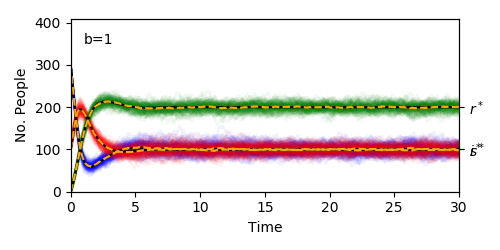
\includegraphics[width=9cm]{figs/prob_b_varb_1.png}}
  \subfloat{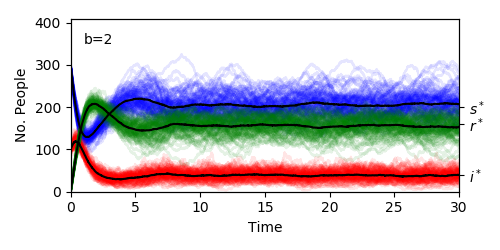
\includegraphics[width=9cm]{figs/prob_b_varb_2.png}}
  \\
  \subfloat{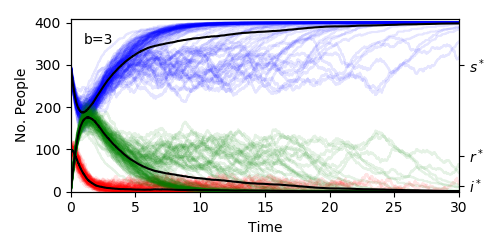
\includegraphics[width=9cm]{figs/prob_b_varb_3.png}}
  \subfloat{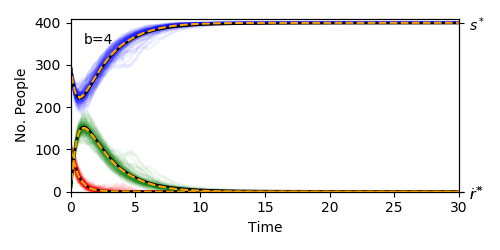
\includegraphics[width=9cm]{figs/prob_b_varb_4.png}}
  \caption{fig:a b plots}
\end{figure*}

\begin{figure*}
  \centering
  \subfloat{
\includegraphics[width=9cm]{figs/prob_ab_legend.pdf}}
  \\
  \subfloat{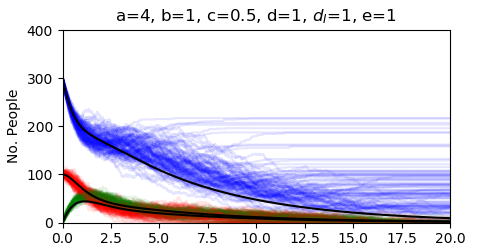
\includegraphics[width=9cm]{figs/prob_c_fig_0.png}}
  \subfloat{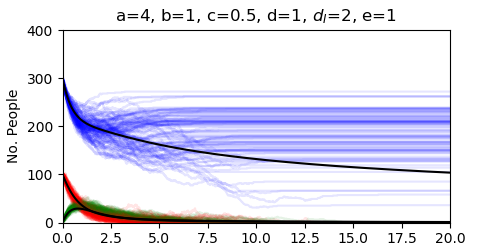
\includegraphics[width=9cm]{figs/prob_c_fig_1.png}}
  \\
  \subfloat{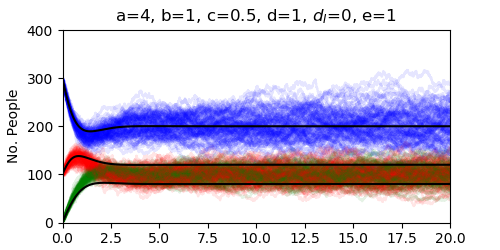
\includegraphics[width=9cm]{figs/prob_c_fig_2.png}}
  \subfloat{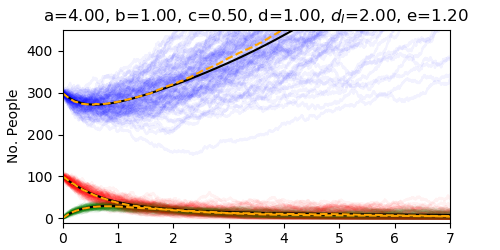
\includegraphics[width=9cm]{figs/prob_c_fig_3.png}}

  \caption{\label{fig:prob_c}}
  
\end{figure*}


\begin{figure*}
  \centering
  \subfloat{
\includegraphics[width=9cm]{figs/prob_ab_legend.pdf}}
  \\
  \subfloat{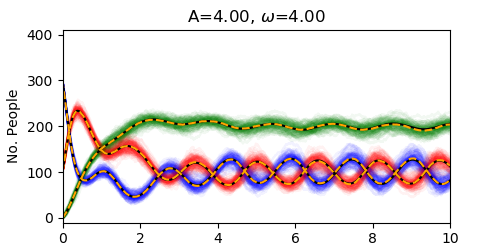
\includegraphics[width=9cm]{figs/prob_d_fig_0.png}}
  \subfloat{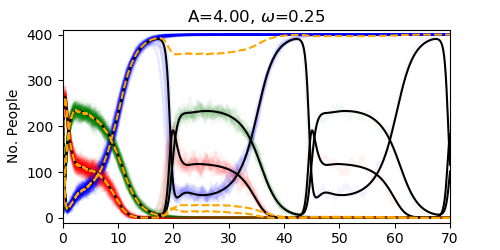
\includegraphics[width=9cm]{figs/prob_d_fig_1.png}}
  \\
  \subfloat{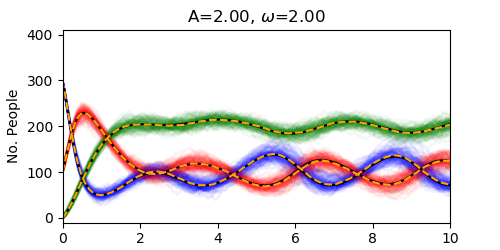
\includegraphics[width=9cm]{figs/prob_d_fig_2.png}}
  \subfloat{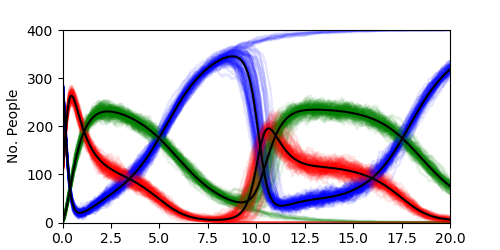
\includegraphics[width=9cm]{figs/prob_d_fig_3.png}}

  \caption{\label{fig:prob_d}}
  
\end{figure*}


\begin{figure*}
  \centering
  \subfloat{
\includegraphics[width=9cm]{figs/prob_ab_legend.pdf}}
  \\
  \subfloat{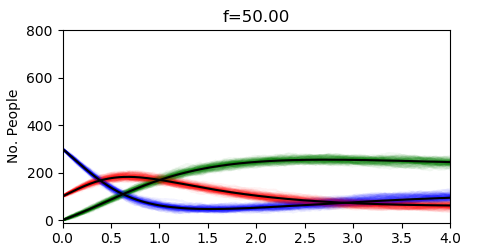
\includegraphics[width=9cm]{figs/prob_e_fig_0.png}}
  \subfloat{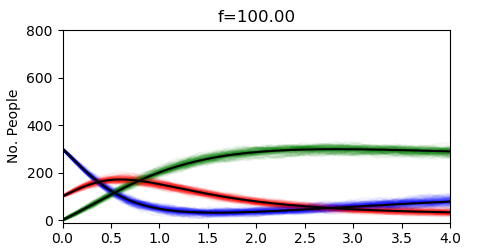
\includegraphics[width=9cm]{figs/prob_e_fig_1.png}}
  \\
  \subfloat{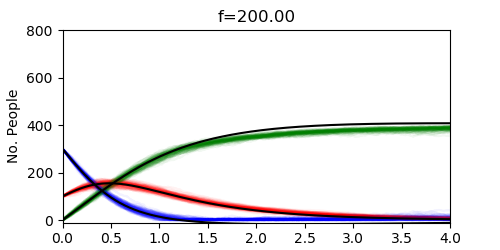
\includegraphics[width=9cm]{figs/prob_e_fig_2.png}}
  \subfloat{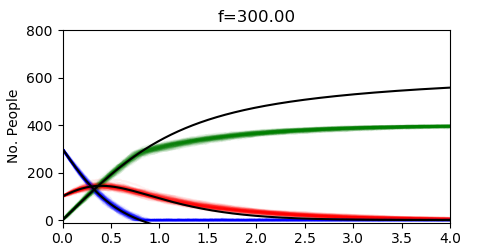
\includegraphics[width=9cm]{figs/prob_e_fig_3.png}}

  \caption{\label{fig:prob_e}}
  
\end{figure*}

\section{Conclusions}

  The obvious next step in the analysis of the SIRS model, and the different features we have discussed is to consider the combination of all of these added features, described by

  \begin{align}
     \begin{split}
        S' &= cR - \qty(A\cos(\omega t) + a_0)\frac{SI}{N} - dS + eN - f \\
        I' &= \qty(A\cos(\omega t)+a_0)\frac{SI}{N} - bI  - (d + d_I)I \\
        R' &= bI - cR - dR + f
     \end{split}
  \end{align} 
   Whilst the implementation of this model trivial\footnote{Armed with the experience of implementing, and understanding the individual features}, the analysis of it is likely a much more complicated due to how the different features will interact with each other. 

\bibliography{../bibliography.bib}


\end{document}  